\documentclass[../main]{subfiles}
\begin{document}

\chapter{Public-Key Encryption}

\begin{theorem}
    Every PK encryption scheme $\Pi$ which is secure against passive attacks is secure also against active attacks.
\end{theorem}

\paragraph{Proof}
    Write two algorithms $PubK^{eav}$ and $PubK^{CPA}$.
    Red arrows, $A$ can make calls to an oracle for $Enc_{pk}(\cdot)$.
    The theorem can be proved by reduction.
    In particular, suppose an adversary $A$ is able to break $\Pi$ with respect to $PubK^{CPA}$ and let us see how out of $A$ one can
    buil an adversary $B$ winning against $\Pi$ int the senso of $PubK^{eav}$.
    \begin{figure}[H]
        \centering
        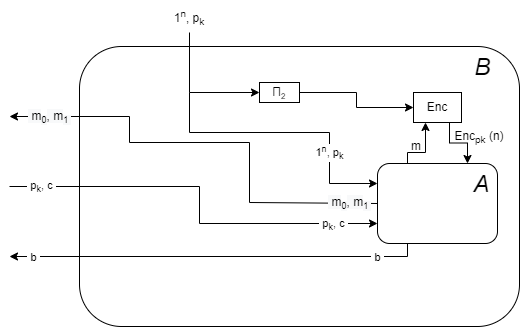
\includegraphics[width=0.7\textwidth]{images/security_of_public_key_passive_attacks}
        \caption{How $\mathcal{B}$ can be generated out of an attacker $\mathcal{A}.$}
    \end{figure}
    Clearly, for obvious reasons
    $$Pr(PubK^{eav}_{\Pi, B}(n) = 1) = Pr(PubK^{CPA}_{\Pi, A}(n) = 1)$$

\begin{theorem}
    Suppose the DDH assumption holds with respect to $GenCG$.
    Then the Elgamal encryption scheme is secure. % All of active or passice attacks
\end{theorem}

\paragraph{Proof}
    Let us consider, just for the sake of this proof, a variation $\tilde{\Pi}$ of the Elgamal encryption scheme $\Pi$ in which $Gen$ is
    defined as usual, while $\tilde{Enc}$ is substantially different
    \newline
    \noindent
    $\textbf{$\tilde{Enc}$} ((\mathcal{G}, q, g, g^x), m):$\\
    $\quad{} y \leftarrow{} \mathbb{Z}_q$\\
    $\quad{} z \leftarrow{} \mathbb{Z}_q$\\
    $\quad{} \textit{return} \; (g^y, g^z, m) $
    \begin{itemize}
        \item What we have designed is completely useless as an encryption scheme, although it will turn out to be useful in this proof.
        \item Let us ask ourselves how the following quantity look like, $$Pr(PubK^{eav}_{\tilde{\Pi}, A}(n) = 1) = \frac{1}{2} \quad\quad \textcolor{red}{(*)}$$
              the challenge ciphertext contains \underline{no information} abount $m_b$
        \item Now we are in a position to build the actual reduction: from an adversary $\mathcal{A}$ winning over Elgamal, we build an adversary
              breaking DDH, call it $\mathcal{B}$
              \begin{figure}[H]
                \centering
                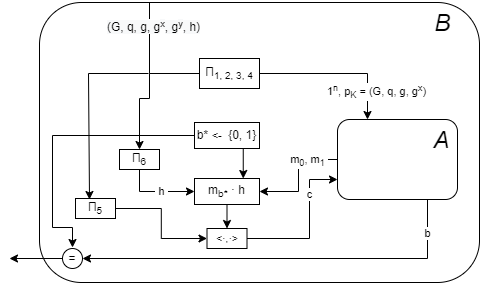
\includegraphics[width=0.7\textwidth]{images/security_of_elgamal_scheme}
                \caption{How $\mathcal{B}$ can be generated out of an attacker $\mathcal{A}.$}
              \end{figure}
        \item What can we say about the behaviours of $\mathcal{A}$ and $\mathcal{B}$. As usual, by construction, $\mathcal{B}$ is designed to cheat $\mathcal{B}$ and make it
              believe he is actually interacting with an experiment. Indeed
              $$Pr(PubK^{eav}_{\tilde{\Pi}, \mathcal{A}}(n) = 1) = Pr(\mathcal{B}(\mathbb{G}, q, g, g^x, g^y, g^z) = 1)$$
              $$Pr(PubK^{eav}_{\Pi, \mathcal{A}}(n) = 1) = Pr(\mathcal{B}(\mathbb{G}, q, g, g^x, g^y, g^{xy}) = 1)$$
        \item This means that the proof is over because
              $$|Pr(\mathcal{B}(\mathbb{G}, \ldots, g^z) = 1) - Pr(\mathcal{B}(\mathbb{G}, \ldots, g^{xy}) = 1)|$$
              $$ = |Pr(PubK^{eav}_{\tilde{\Pi}, \mathcal{A}} (n) = 1) - Pr(PubK^{eav}_{\Pi, \mathcal{A}} (n) = 1)|$$
              $$ \textcolor{red}{(*)} = | \frac{1}{2} - (\frac{1}{2} + \varepsilon (n))|$$
              $$ = |- \varepsilon (n)| = \varepsilon (n)$$
              where $\varepsilon$ is \underline{NOT} negligible.
    \end{itemize}
\end{document}	